\documentclass[tikz]{standalone}
\usepackage{tikz-3dplot}
\begin{document}
    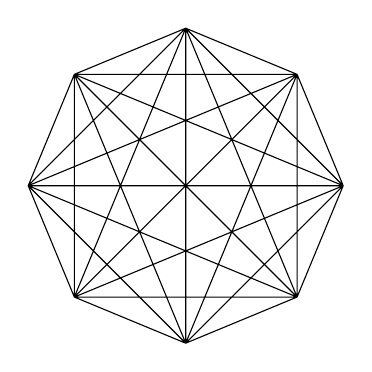
\begin{tikzpicture}[scale=1,line join=round]
    \path 
    \foreach \x in {0, 1} 
    \foreach \y in {0, 1} 
    \foreach \z in {0, 1} 
    {coordinate(\x\y\z) at (180*\x+90*\y+45*\z:2) };
    \draw
    \foreach \xa in {0, 1}
    \foreach \xb in {0, 1}
    \foreach \ya in {0, 1}
    \foreach \yb in {0, 1}
    \foreach \za in {0, 1}
    \foreach \zb in {0, 1}
    {(\xa\ya\za) -- (\xb\yb\zb)};
\end{tikzpicture}
\end{document}
